%\documentclass[14pt, notes]{beamer}
\documentclass[14pt]{beamer}

%\usepackage{pgfpages}
%\setbeameroption{show notes}
%\setbeameroption{show notes on second screen=right}

%encoding
\usepackage[utf8]{inputenc}

%language
\usepackage[russian]{babel}
\usepackage{amsmath}
\usepackage{bm}
\usepackage{graphicx}
\usepackage{hyperref}
\graphicspath{{images/}}%путь к рисункам

\setbeamerfont{author in head/foot}{size=\small}
\setbeamerfont{title in head/foot}{size=\footnotesize}

\title[Моделирование динамики жидкости в сосудах]{Моделирование динамики жидкости в крупных кровеносных сосудах}
\date{\today}
\author{Долгов Д.А.}
\institute{Кемеровский Государственный Университет \\
    \vspace{0.7cm}
    \vspace{0.7cm}
} 
\usetheme[numbers, totalnumbers, minimal, nologo]{Statmod}
% Привычный шрифт для математических формул
\usefonttheme[onlymath]{serif}

\definecolor{statmodblue}{RGB}{100,10,30}
\definecolor{statmodsand}{RGB}{244,215,103}

\begin{document}
\maketitle

%description of the problem
\begin{frame}
\frametitle{Введение}
Рассмотрим задачу о течении крови внутри крупных сосудов с гибкими стенками и клапанами. Кровь будем моделировать как вязкую, несжимаемую однородную жидкость, стенки сосуда и лепестки клапанов - как поверхность заданной формы, обладающую определенной жесткостью.
\end{frame}

%description of the problem: schema
\begin{frame}
\frametitle{Введение}
    \begin{center}
        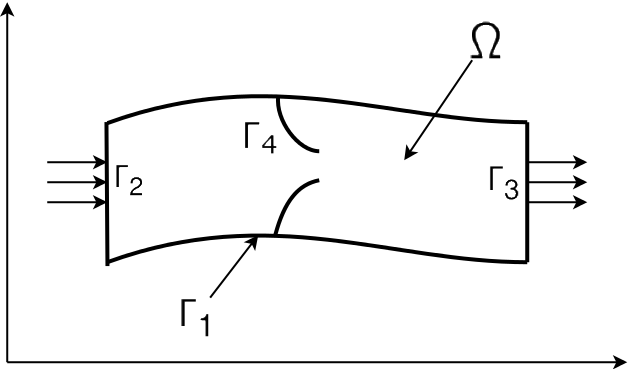
\includegraphics[width=9cm]{area.png}
    \end{center}
\end{frame}
\note{$\Gamma_1,\Gamma_4$ - гибкие стенки, $\Gamma_2,\Gamma_3$ - вход/выход}

% navier stokes equations
\begin{frame}
\frametitle{Моделирование течения}
Система уравнений Навье-Стокса:
\begin{gather}
    \label{eq:motion}
    \rho ( \frac{\partial u}{\partial t} + u \cdot \nabla u) = - \nabla p + \nabla \sigma + f\\
    \label{eq:continuity}
    \nabla u = 0 
\end{gather}
где $\sigma = \mu (\nabla u + (\nabla u)^{T}$, с начальными условиями
\begin{gather}
    u(x, y, z, t_0) = 0,\;p(x, y, z, t_0) = p_0
\end{gather}

\end{frame}
\note{Уравнения записаны в векторном виде, $\sigma$ - вязкий тензор напряжений}

% boundary
\begin{frame}
\frametitle{Условия на стенках}
\begin{itemize}
    \item на $\Gamma_1,\Gamma_4$ задаются условия прилипания
    \item на $\Gamma_2,\Gamma_3$ заданы значения давления $P_{int},P_{out}$
\end{itemize}

Помимо этого в каждой точке стенки определена сила сопротивления деформации
\begin{equation*}
    \label{eq:define_boundary_force}
    F = F(x, y, z, t)
\end{equation*}

\end{frame}
\note{Условие прилипания в данном случае означает, что граница будет двигаться с той же скоростью, что и жидкость}

% solve method 
\begin{frame}
\frametitle{Метод решения}
В соответствии с методом погруженной границы, будем рассматривать отдельно задачи вычисления параметров течения жидкости и параметров движения стенок сосуда и клапанов. Для этого введем в расчетной области сетки:
\begin{itemize}
    \item $\Omega = \Omega(x, y, z)$ - равномерная разнесенная сетка для расчета течения
    \item $\Gamma = \Gamma(q, r, s, t)$ - соответствует стенкам сосуда и клапанам в лагранжевых координатах
\end{itemize}

\end{frame}

% solve method: diagram
\begin{frame}
\frametitle{Метод решения}
    \begin{center}
        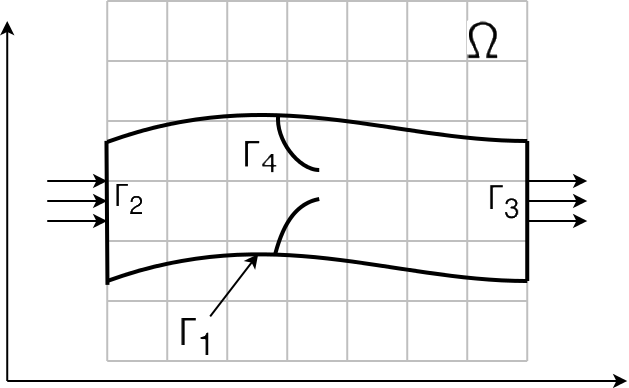
\includegraphics[width=9cm]{area_ibm.png}
    \end{center}
\end{frame}

% solve method: ibm 
\begin{frame}
\frametitle{Алгоритм решения}
\setbeamercolor{normal text}{fg=gray,bg=}
\setbeamercolor{alerted text}{fg=black,bg=}
\usebeamercolor{normal text}
    \begin{itemize}
        \item \alert<+>{Рассчитываем параметры течения в $\Omega(x, y, z)$, в частности векторное поле скорости}
        \item \alert<+>{С помощью полученной скорости вычислить скорость движения точек границы и ее деформацию}
        \item \alert<+>{На основе деформации $\Gamma(q, r, s, t)$ находим силу сопротивления $F(q, r, s, t)$}
        \item \alert<+>{С помощью $F(q, r, s, t)$ вычислить $f(x, y, z, t)$ для жидкости}
        \item \alert<+>{Перейти к новому временному слою с измененной $f(x, y, z, t)$}
    \end{itemize}
\end{frame}

% solve method:split scheme
\begin{frame}
\frametitle{Схема расщепления}
\begin{gather}
    \label{eq:split_first}
    \frac{u^* - u^n}{\triangle t} = - (u^n \cdot \nabla) u^n + \frac{1}{\rho} \nabla \sigma + f\\
    \label{eq:split_second}
    \rho \triangle p^{n+1} - (\nabla p \cdot \nabla p^{n+1}) = \frac{\rho^2 \nabla u^*}{\triangle t}\\
    \label{eq:split_third}
    \frac{u^{n+1} - u^*}{\triangle t} = - \frac{1}{\rho} \nabla p^{n+1}
\end{gather}
где $\nabla \sigma (u^n, \mu) = \mu \triangle u^n + (\nabla \mu \cdot \nabla) u^n + (\nabla \mu \cdot J_{u^n}) $
\end{frame}

% solve method:split algorithm 
\begin{frame}
\frametitle{Алгоритм решения}
\setbeamercolor{normal text}{fg=gray,bg=}
\setbeamercolor{alerted text}{fg=black,bg=}
\usebeamercolor{normal text}
    \begin{itemize}
        \item \alert<+>{С помощью схемы стабилизирующей поправки решаем уравнение \eqref{eq:split_first} и получаем промежуточное поле скорости $u^*$}
        \item \alert<+>{Из уравнения \eqref{eq:split_second} методом бисопряженных градиентов определяем поле давления}
        \item \alert<+>{Восстанавливаем окончательное поле вектора скорости по явным формулам \eqref{eq:split_third}}
    \end{itemize}
\end{frame}

% solve method:immersed boundary
\begin{frame}
\frametitle{Погруженная граница}
Взаимодействие погруженной границы и жидкости:
\begin{gather}
    \label{eq:ibm_velocity}
    \frac{\partial X}{\partial t} = \int_{\Gamma} u \cdot \delta (x - X)\; dx\; dy\; dz \\
    \label{eq:ibm_force}
    f = \int_{\Omega} F \cdot \delta (x - X)\; dq\; dr\; ds
\end{gather}
и условия прилипания
\begin{gather}
    \label{eq:no_slip}
    \frac{\partial X}{\partial t} (q, r, s, t) = u(X(q, r, s, t), t)
\end{gather}
\end{frame}
\note{Заглавные символы относятся к погруженной границе, обычные - к жидкости}

% totals and examples
\begin{frame}
\frametitle{Метод решения}
Данный метод разрабатывался с учетом применения в исследовании биологических систем, для которых подвижность и эластичность границ является важным фактором.
Он разделяет одну сложную задачу на три более простые - моделирование течения, моделирование состояния границы и их взаимодействие.
\end{frame}

% totals and examples
\begin{frame}
\frametitle{Метод решения}
Это позволяет применять мощные методы для решения каждой из задач. Помимо этого такой подход позволяет единообразно моделировать различные классы проблем, т.к. погруженная граница может иметь практически любую форму.
\end{frame}

% totals and examples
\begin{frame}
\frametitle{Метод решения}
Метод погруженной границы пока не реализован ни в одном из крупных CFD пакетов (такая работа начата только в OpenFOAM, но она находится на стадии обсуждения сообществом).
\end{frame}

% totals and examples
\begin{frame}
\frametitle{Работы других коллективов}
\begin{itemize}
    \item IBAMR (UNC McAllister Heart Institute)
    \item \href{run:video/valve\_flow\_side.avi}{Пример моделирования аортального клапана}
    \item \href{run:video/MV\_side.avi}{Расчет параметров хордового протеза для митрального клапана}
\end{itemize}
\end{frame}

% totals and examples
\begin{frame}
\frametitle{Примеры}
\begin{itemize}
    \item \href{run:video/cylinder1.avi}{Деформация стенок сосуда}
    \item \href{run:video/cylinder2.avi}{Аналогичный расчет на более мелкой сетке}
\end{itemize}
\end{frame}

\begin{frame}
\frametitle{Дополнительная информация}
    \begin{itemize}
        \item Peskin C.S., Numerical Analysis of Blood Flow in the Heart// JCP 25,220-252, (1977)
        \item Peskin C.S., The immersed boundary method, (1977)
        \item Mittal R, Iaccarino G, Immersed boundary method// ARFM, 37, 239-261, (2005)
        \item Bandringa H., Immersed boundary method, Groningen, (2010)
        \item Kruger T., Introduction to the immersed boundary method, (2011)
    \end{itemize}
\end{frame}
\note{
    \begin{itemize}
        \item Основная работа "непрерывного метода" (journal of computational physic)
        \item Более полная и развернутая
        \item Хороший обзор (Annual Review of Fluid Mechanics)
        \item Обзор в диссертационной работе
        \item Больше практики, но со спецификой другого метода расчета (Lattice Boltzmann method)
    \end{itemize}
}

\end{document}
